\chapter{RESULTS}

\graphicspath{ {./results/} }
%%%%%%%% This line gets rid of page number on first page of text
\thispagestyle{empty}

%%%%%%%%%%%%%

The result section details essential findings from our research study and prototype testing, including multiple iterations and user testing to analyze different variations.

\section{Visual Analysis}

The critical finding from the research highlights that the representations learned by the VGG16 image recognition model are highly amenable to visualization, in large part because they are representations of visual concepts. Although a wide variety of techniques are under development in the research and visual analytics community, we covered three of the most accessible and useful ones:

\begin{enumerate}
\item Visualizing heatmaps of class activation
\item Visualizing filter patterns
%\item Visualizing intermediate activations
\end{enumerate}

For all three methods, we use the VGG16 model, a convolutional neural network based model trained on the imagenet database that we introduced in the previous section.

\section*{Image Receptiveness}

This step helps to understand precisely which part of an image identified to belong to a specific class or category (class names known to VGG16), and thus allows localizing objects in images.

We feed the following image of a group of bee-eater sitting on a tree branch as an input image.

%Input image ~\ref{fig:myFig}.
\begin{figure}[htbp]
\centering
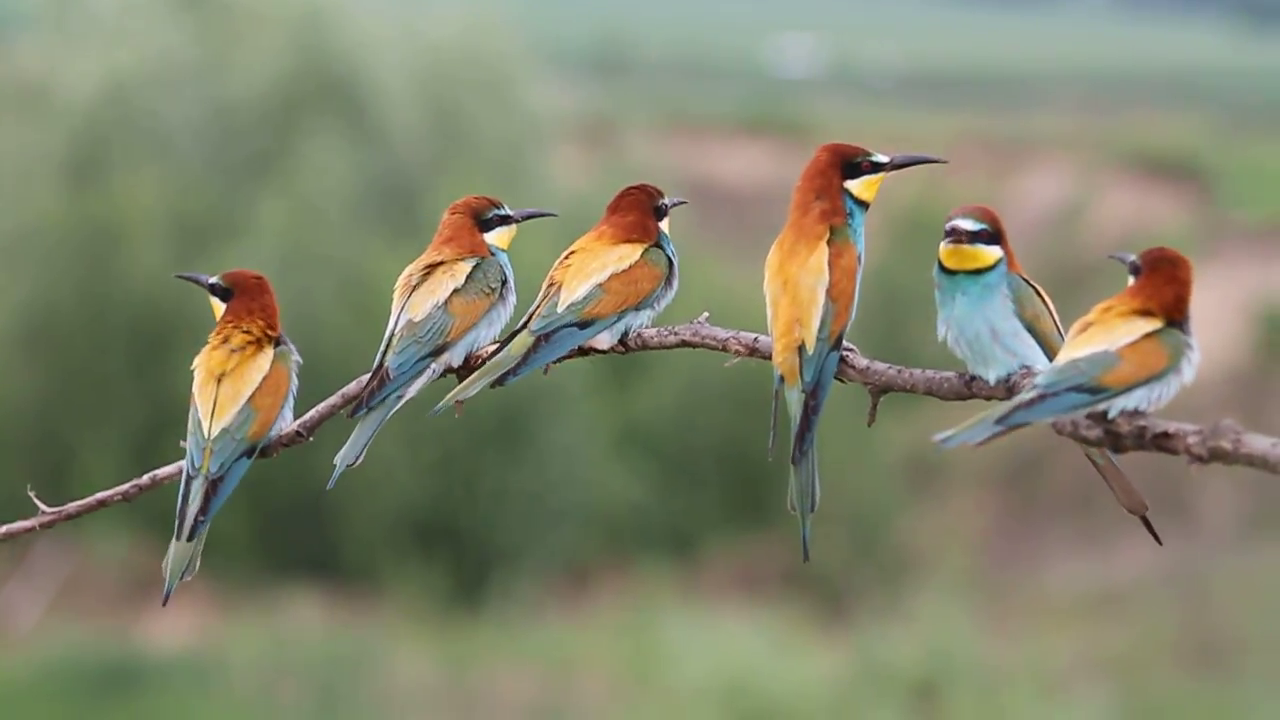
\includegraphics[width=0.80\textwidth]{images/colorful-group-of-birds-get-together_vkmuak6_e__F0000.png}
\caption{An image of colorful group of birds uploaded by the user}
\label{fig:myFig}
\end{figure}

%Class activation heatmap~\ref{fig:heatmap-1}.
\begin{figure}[htbp]
\centering
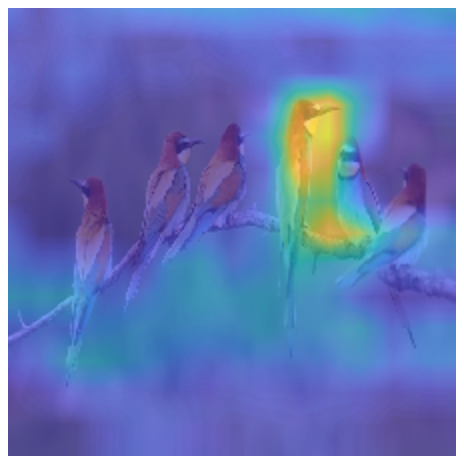
\includegraphics[width=0.50\textwidth]{images/heatmap-class-activations.png}
\caption{Image Receptivity}
\label{fig:heatmap-1}
\end{figure}

\section*{Activation Graph}

This step helped to understand when fed with an input image, how successful layers of the network transformed the input image. It also helped get an idea of the meaning of the individual network filters.

Our visualization technique helped to answer two important questions:

\begin{itemize}
\item  Why did the network think this image contained a bee-eater?
\item Where is the bee-eater located in the picture?
\end{itemize}

In particular, what is most exciting to note is that the head region of the fourth bird, which is the largest of all six birds are strongly activated: this is probably how the network can tell the difference between bee-eater and any other bird.

%\section{User Study}

\iffalse
\section{Visualization Outcome}
\section{Statistical Analysis}
\section{Visual Analysis}


\section{User Testing}
\section{Performance Testing}
\fi
